\documentclass[border=3pt]{standalone}
\usepackage{tikz}
\usetikzlibrary{arrows.meta,calc,positioning}
\tikzset{pin/.style={-{Stealth[length=5pt]}},
  blk/.style={draw, thick, minimum width=16mm, minimum height=14mm, font=\sffamily\small, align=center},
  preg/.style={draw, thick, fill=black!8, minimum width=3mm, minimum height=30mm}}
\begin{document}
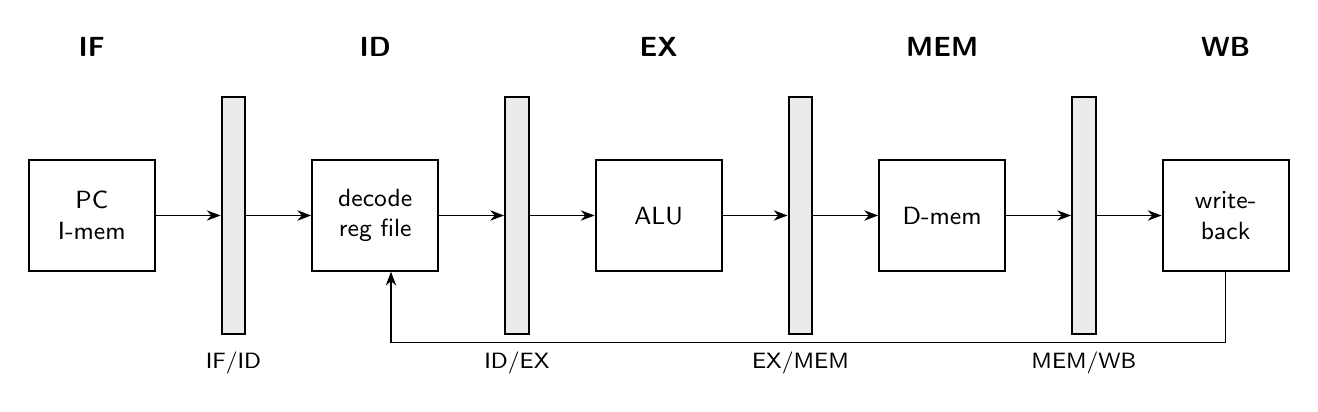
\begin{tikzpicture}[font=\sffamily\small]
  % stage blocks
  \node[blk] (if)  at (0,0)    {PC\\I-mem};
  \node[preg] (p1) at (1.8,0)  {};
  \node[blk] (id)  at (3.6,0)  {decode\\reg file};
  \node[preg] (p2) at (5.4,0)  {};
  \node[blk] (ex)  at (7.2,0)  {ALU};
  \node[preg] (p3) at (9.0,0)  {};
  \node[blk] (mem) at (10.8,0) {D-mem};
  \node[preg] (p4) at (12.6,0) {};
  \node[blk] (wb)  at (14.4,0) {write-\\back};
  % datapath
  \draw[pin] (if.east) -- (p1.west |- if.east);
  \draw[pin] (p1.east |- id.west) -- (id.west);
  \draw[pin] (id.east) -- (p2.west |- id.east);
  \draw[pin] (p2.east |- ex.west) -- (ex.west);
  \draw[pin] (ex.east) -- (p3.west |- ex.east);
  \draw[pin] (p3.east |- mem.west) -- (mem.west);
  \draw[pin] (mem.east) -- (p4.west |- mem.east);
  \draw[pin] (p4.east |- wb.west) -- (wb.west);
  % writeback loop into register file
  \draw[pin] (wb.south) -- ++(0,-9mm) -| ($(id.south)+(2mm,0)$);
  % stage labels
  \foreach \n/\l in {if/IF, id/ID, ex/EX, mem/MEM, wb/WB}{
    \node[font=\sffamily\bfseries, above=17mm of \n.center, anchor=south] at (\n |- 0,0.2) {\l};}
  % pipeline register labels
  \foreach \p/\l in {p1/{IF/ID}, p2/{ID/EX}, p3/{EX/MEM}, p4/{MEM/WB}}{
    \node[font=\sffamily\footnotesize, below=1mm of \p.south] {\l};}
\end{tikzpicture}
\end{document}
